\section{How later tokens read a written value}\label{sec:read}

Preregistered results name their prediction (B1 is prediction~1 of preregistration~B; \cref{app:prereg}); the others are marked exploratory or post hoc.

\begin{figure*}[t]
  \centering
  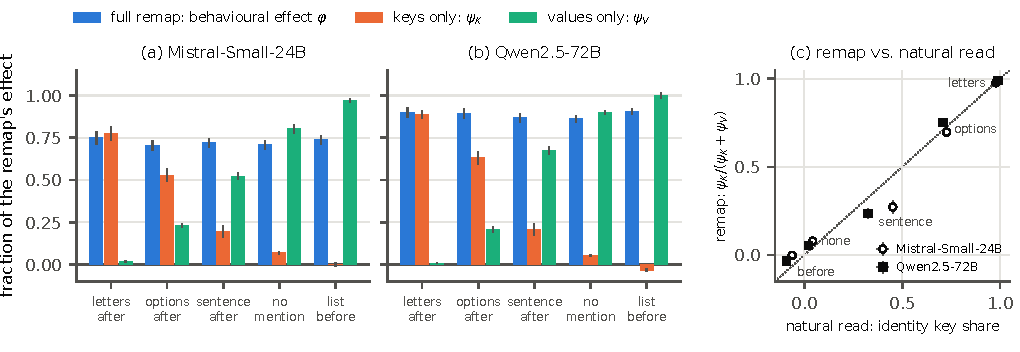
\includegraphics[width=\textwidth]{figures/fig_frames.pdf}
  \caption{\textbf{The same learned intervention has nearly the same behavioural effect in every format, but whether the writing token's keys or its values carry it depends on the later mentions.} The rank-16 DAS remap M of \citet{anonymous2026fitted} against their unfitted PCA patch P (released bases) at Mistral-Small-24B (a) and Qwen2.5-72B (b). Blue: $\varphi$, the shift of M relative to P towards the target T, as a fraction of the natural source-to-target shift (\cref{eq:phi}). Orange: $\psi_K$, the fraction of the M$-$P difference that P reproduces when given M's keys at the writing token (\cref{eq:psik}). Green: $\psi_V$, the same with M's values (\cref{eq:psiv}). Keys or values are exchanged from block~6 on. (a, b)~$n = 96$ story cores with B, S and T distinct, $\times$ 3 fits averaged within core; error bars are 95\% bootstrap intervals over cores. (c)~Exploratory cross-check: the remap's key share $\psi_K/(\psi_K+\psi_V)$ against the identity key share $s_{\mathrm{ID}}$ of the unpatched model in the same format (our stories, same pinned models; dotted line: equality). All values, with the removal fractions $\rho_K$ and $\rho_V$, are in \cref{tab:frames}.}
  \label{fig:frames}
\end{figure*}

\subsection{Later mentions decide which channel carries the value}\label{sec:mentions}

\begin{table}[t]
  \centering
  \caption{\textbf{Position decides the key read.} Instruction-matched $2{\times}2$: the same list or neutral sentence naming every candidate, placed after or before the story, with ``Answer with one word'' in every format; \fmtNone{} for reference. Entries are $\mathrm{ID}_K$ in nats with 95\% bootstrap CIs over $n = 150$ stories, at Qwen2.5-7B and 14B, Mistral-7B and OLMo-2-7B; keys are clamped from layer~0. Preregistration~E (prediction E1).}
  \label{tab:twobytwo}
  \resizebox{\columnwidth}{!}{\footnotesize\setlength{\tabcolsep}{3pt}\begin{tabular}{@{}lcccc@{}}
\toprule
Format & Qwen-7B & Qwen-14B & Mistral-7B & OLMo-2-7B \\
\midrule
\fmtListA & \begin{tabular}[t]{@{}c@{}}+20.6\\[-1pt]{\scriptsize[20.2, 21.0]}\end{tabular} & \begin{tabular}[t]{@{}c@{}}+35.8\\[-1pt]{\scriptsize[34.9, 36.7]}\end{tabular} & \begin{tabular}[t]{@{}c@{}}+15.6\\[-1pt]{\scriptsize[15.1, 16.0]}\end{tabular} & \begin{tabular}[t]{@{}c@{}}+8.7\\[-1pt]{\scriptsize[8.4, 8.9]}\end{tabular} \\
\fmtPost & \begin{tabular}[t]{@{}c@{}}+5.5\\[-1pt]{\scriptsize[5.2, 5.8]}\end{tabular} & \begin{tabular}[t]{@{}c@{}}+12.1\\[-1pt]{\scriptsize[11.5, 12.7]}\end{tabular} & \begin{tabular}[t]{@{}c@{}}+7.9\\[-1pt]{\scriptsize[7.3, 8.4]}\end{tabular} & \begin{tabular}[t]{@{}c@{}}+2.0\\[-1pt]{\scriptsize[1.8, 2.2]}\end{tabular} \\
\fmtBefore & \begin{tabular}[t]{@{}c@{}}-0.1\\[-1pt]{\scriptsize[-0.2, -0.1]}\end{tabular} & \begin{tabular}[t]{@{}c@{}}-0.1\\[-1pt]{\scriptsize[-0.2, -0.0]}\end{tabular} & \begin{tabular}[t]{@{}c@{}}+0.0\\[-1pt]{\scriptsize[-0.1, 0.1]}\end{tabular} & \begin{tabular}[t]{@{}c@{}}-0.3\\[-1pt]{\scriptsize[-0.4, -0.2]}\end{tabular} \\
\fmtSentB & \begin{tabular}[t]{@{}c@{}}-0.0\\[-1pt]{\scriptsize[-0.1, 0.1]}\end{tabular} & \begin{tabular}[t]{@{}c@{}}-0.1\\[-1pt]{\scriptsize[-0.2, 0.0]}\end{tabular} & \begin{tabular}[t]{@{}c@{}}-0.0\\[-1pt]{\scriptsize[-0.1, 0.1]}\end{tabular} & \begin{tabular}[t]{@{}c@{}}-0.2\\[-1pt]{\scriptsize[-0.3, -0.2]}\end{tabular} \\
\midrule
\fmtNone & \begin{tabular}[t]{@{}c@{}}+1.0\\[-1pt]{\scriptsize[0.9, 1.2]}\end{tabular} & \begin{tabular}[t]{@{}c@{}}+1.1\\[-1pt]{\scriptsize[0.9, 1.2]}\end{tabular} & \begin{tabular}[t]{@{}c@{}}+0.6\\[-1pt]{\scriptsize[0.5, 0.6]}\end{tabular} & \begin{tabular}[t]{@{}c@{}}+0.4\\[-1pt]{\scriptsize[0.3, 0.5]}\end{tabular} \\
\bottomrule
\end{tabular}
}
\end{table}


\paragraph{Natural formats.}
\Cref{tab:natural} gives $\mathrm{ID}_K$ for every format in all \nModels{} models, and \cref{fig:formats} summarises it relative to \fmtOpt{} (both in the appendix). The formats fall into three regimes.

\emph{Candidates listed after the writing token.} Under \fmtOpt{} and \fmtLetter{}, $\mathrm{ID}_K$ is large and positive in every model, from \idKOptQwenOnefive{} nats at Qwen2.5-1.5B to \idKOptQwenFourteen{} nats at Qwen2.5-14B under \fmtOpt{}. This was preregistered at 1.5B on fresh stories (A1) and in five held-out models from 3B to 8B (B1); both were met. At Qwen2.5-14B and at 24--72B it is exploratory. Under \fmtLetter{}, the value channel then carries little identity: $\mathrm{ID}_V$ is at most about one nat in every model (exploratory; \cref{tab:decomposition}).

\emph{No later mention.} Under \fmtNone{}, $\mathrm{ID}_K$ is at most \noneMax{} nats, less than a tenth of its \fmtOpt{} value in every model, and the paired \fmtOpt{}$-$\fmtNone{} difference is positive in 5/5 held-out models (B2, met). The identity is copied instead: $\mathrm{ID}_V$ under \fmtNone{} exceeds $\mathrm{ID}_K$ more than tenfold in every model (exploratory; \cref{tab:decomposition}). The residual key identity is small but not zero; in four models from 7B up (Qwen2.5-7B, 14B and 32B and Qwen3-8B) its interval extends just beyond the $\pm 1$-nat equivalence margin that preregistration~A set at 1.5B, which we report as an unpredicted observation. \fmtBefore{} names the same candidates as \fmtOpt{}, but before the writing token, where the causal mask prevents them from attending to it. Its $\mathrm{ID}_K$ is never reliably positive: it is negative in nine of the ten models, most strongly at Qwen2.5-72B ($\idKBeforeQwenSeventytwo$ nats), and indistinguishable from zero at Mistral-7B. The $\leq 0.5$-nat bound was preregistered for the three largest models (C4, second part) and met. We have no tested explanation for the negative sign.

\emph{A neutral sentence after the story.} \fmtPost{} names all six candidates in a plain sentence and asks for a free-form answer. At Qwen2.5-1.5B and 3B it carries no positive key identity: it is slightly negative at 1.5B ($\idKPostQwenOnefive$ nats) and indistinguishable from zero at 3B (\cref{tab:natural}). From 7B up it carries an intermediate amount in every model, from \idKPostOlmoSeven{} nats at OLMo-2-7B to \idKPostQwenFourteen{} at Qwen2.5-14B. This was not predicted, and it refutes the narrower ``listed options only'' account we had formed post hoc at 1.5B (\cref{sec:discussion}, limitation~ii). Across all formats, with clamps from layer~0, the effects of clamping the key and the value add up, with a small interaction (exploratory; \cref{tab:decomposition}). Because nats grow with the model's confidence, the scale-free identity key share $s_{\mathrm{ID}}$ is the fairer comparison across models: above 1.5B it is \idShareLetterMinNoOnefive{}--\idShareLetterMax{} under \fmtLetter{}, \idShareOptMinNoOnefive{}--\idShareOptMax{} under \fmtOpt{}, at most \idSharePostMax{} under \fmtPost{}, at most \idShareNoneMax{} under \fmtNone{} and at most \idShareBeforeMax{} under \fmtBefore{} (exploratory; \cref{tab:idshare}).

\paragraph{An instruction-matched $2{\times}2$.}
The natural formats differ in more than position: \fmtOpt{} asks for ``exactly one choice'', and a list is not a sentence. Preregistration~E therefore crosses \{list, sentence\} with \{before, after\}, with the same one-word instruction in every format (\cref{tab:twobytwo}). All parts of E1 were met. $\mathrm{ID}_K$ is \twoAfterMin{}--\twoAfterMax{} nats under \fmtListA{}, close to the \fmtOpt{} value in the same model, and \twoPostMin{}--\twoPostMax{} under \fmtPost{}. Under \fmtBefore{} and \fmtSentB{}, every CI contains zero or lies below it. The paired differences \fmtListA{}$-$\fmtBefore{} and \fmtPost{}$-$\fmtSentB{} are positive, with CIs excluding zero, in 4/4 models. Moving the same words from before the writing token to after it switches the key read on, for a list and for a sentence alike. Position, not the instruction or the list format, decides whether the key channel opens. The list format changes only how far it opens: in all four models $\mathrm{ID}_K$ is larger under \fmtListA{} than under \fmtPost{}, a comparison we did not preregister.

\subsection{Across tasks, families and scale}\label{sec:general}

\paragraph{Tasks.}
On the paint and schedule tasks, in five models of 7--14B parameters (\cref{tab:tasks}), $\mathrm{ID}_K$ under \fmtOpt{} is \taskPaintOptMin{}--\taskPaintOptMax{} nats (paint) and \taskScheduleOptMin{}--\taskScheduleOptMax{} nats (schedule). The paired \fmtOpt{}$-$\fmtNone{} difference is positive in 5/5 models per task (D1, met). Under \fmtBefore{}, $\mathrm{ID}_K$ is at most \taskPaintBeforeMax{} and \taskScheduleBeforeMax{} nats, within the preregistered 0.5-nat bound in 10/10 task--model cells (D2, met). \fmtPost{} again lies between \fmtNone{} and \fmtOpt{} in every model (exploratory).

\begin{figure}[t]
  \centering
  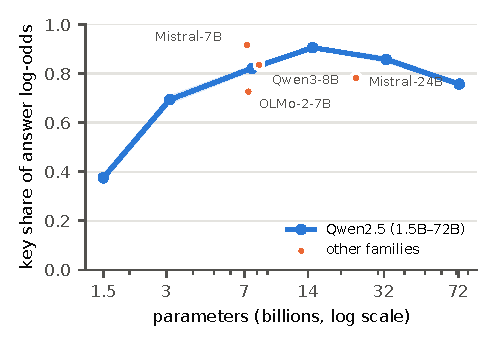
\includegraphics[width=\columnwidth]{figures/fig_scale.pdf}
  \caption{\textbf{Key share of the \fmtOpt{} answer across scale and families.} $s_K = \bar d_K/(\bar d_K + \bar d_V)$ with keys and values clamped from layer~0. Line and band: Qwen2.5-Instruct 1.5B--72B with 95\% bootstrap CIs; points: other families. $n = 150$ stories per model; values with CIs in \cref{tab:natural}. $s_K$, the preregistered measure, includes non-specific effects; the identity key share $s_{\mathrm{ID}}$ shows the same rise to 14B and fall beyond (\cref{tab:idshare}).}
  \label{fig:scale}
\end{figure}

\paragraph{Scale and families.}
Within Qwen2.5, the \fmtOpt{} key share rises from \shareQwenOnefive{} at 1.5B through \shareQwenThree{} (3B) and \shareQwenSeven{} (7B) to \shareQwenFourteen{} at 14B, then falls to \shareQwenThirtytwo{} at 32B and \shareQwenSeventytwo{} at 72B (\cref{fig:scale}); the 14B and 72B intervals do not overlap. The size trend was exploratory (B3), and the preregistered threshold $s_K \geq 0.80$ for the three largest models was met only at 32B (C4; \cref{sec:failed}). Because the 32B and 72B runs used a different software version and two GPUs, preregistration~E re-ran Qwen2.5-14B in the large-model setup and Qwen2.5-32B in the small-model setup. The re-runs gave \shareEnvFourteen{} and \shareEnvThirtytwo{}, the same as the originals to two decimals (E3, met). The fall beyond 14B is therefore not an artefact of the environment, and it is also seen in the identity key share (\idShareOptQwenFourteen{} at 14B, \idShareOptQwenSeventytwo{} at 72B), although we do not know its cause. The other families give similar shares (\shareOlmoSeven{}--\shareMistralSeven{}; \cref{fig:scale}), and every model except Qwen2.5-1.5B carries more than half of the \fmtOpt{} effect in the key.

\paragraph{Depth.}
At layer~0 a key is a function of the input token embedding alone. To check whether the read is confined to the lowest layers' keys, an exploratory onset sweep starts both clamps deeper (\cref{tab:onset}). With $\ell_0 \approx 0.06L$ the shares are unchanged to two decimals in eight of ten models. With $\ell_0 \approx 0.3L$, which leaves the keys and values of about the lowest 30\% of the layers at the base run's, the share stays at or above one half in seven of the ten models (up to \onsetLateQwenFourteen{} at Qwen2.5-14B). It falls below one half at Qwen2.5-1.5B (\onsetLateQwenOnefive{}) and Mistral-24B (\onsetLateMistralTwentyfour{}), and almost to zero at OLMo-2-7B (\onsetLateOlmoSeven{}), where the key effect depends on the lowest layers. At this onset the clamp is no longer exact and the key and value effects no longer add up, so these shares are descriptive only (\cref{app:additional}); deeper keys are still computed from a residual stream that contains the written word.


\subsection{Which later tokens read the writing token's key}\label{sec:readers}

\begin{figure*}[t]
  \centering
  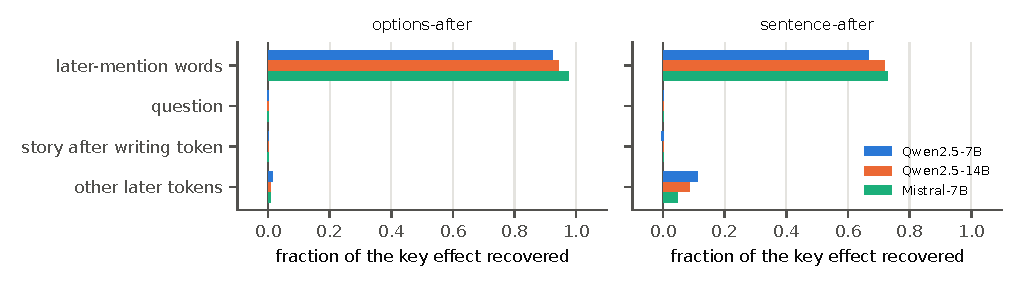
\includegraphics[width=\textwidth]{figures/fig_localisation.pdf}
  \caption{\textbf{The later mentions read the writing token's key.} Exact row-restricted splice at Qwen2.5-7B, Qwen2.5-14B and Mistral-7B ($n = 60$ stories). Only the listed group of later tokens sees the source key at the writing token, in every layer, while all other tokens see the base key. Bars give the fraction of the full key effect (all tokens see the source key) that this recovers, as a ratio of mean log-odds changes. Left, \fmtOpt{}: the later-mention words are the listed options. Right, \fmtPost{}: they are the candidate words of the neutral sentence. ``Other later tokens'' covers the instruction, chat template, prefill and answer position. Preregistration~D (prediction D3); values in \cref{tab:localisation}.}
  \label{fig:localisation}
\end{figure*}


Which later tokens read the writing token's key? With the row-restricted splice (\cref{sec:method}), we let only one group of later tokens see the source key (\cref{fig:localisation}). Under \fmtOpt{}, the option words alone recover \locScaleOptMin{}--\locScaleOptMax{} of the full key effect at 7--14B. The question, the story after the writing token and the remaining tokens, including the answer position, each recover at most \locScaleOptOtherMax{}. Under \fmtPost{}, the candidate words of the neutral sentence recover \locScalePostMin{}--\locScalePostMax{} and the other later tokens \locScalePostOtherMin{}--\locScalePostOtherMax{}; \locScalePostLeftMin{}--\locScalePostLeftMax{} is not recovered by any single group, so the groups do not add up (\cref{tab:localisation}). Both parts of D3 were met in 3/3 models. We did not localise the read at 24B or 72B. Under \fmtOpt{}, then, the answer position gains almost nothing from seeing the source key itself, which fits a two-step account: the key changes what the later mentions retrieve, and the answer then reads the later mentions. We did not test the second step directly.

An exploratory run at Qwen2.5-1.5B agrees, and places the read in middle layers (\cref{app:additional}).

\subsection{Identity, not belief role}\label{sec:role}

A later \emph{shelf} that attends to an earlier \emph{shelf} is duplicate-token attention, the pattern of the duplicate-token heads described by \citet{wang2022ioi}. The key read is an identity lookup of this kind, and we claim nothing more for it: each value is a single word, so ``identity'' means the lexical identity of that word in its context, and the read is not confined to the lowest layers' keys (\cref{sec:general}). We did not identify the heads that perform it.

Could the writing token's channels carry more than identity, such as whether the person asked about saw the move? The role-swap control exchanges the observer's and the non-observer's names but keeps the location word. This shifts the belief answer by \roleEffMin{} to \roleEffMax{} nats, depending on model and format (\cref{tab:role}). Clamping the writing token's key or value alone to the role-swapped run carries at most \roleFracMax{} of that shift, under \fmtOpt{}, \fmtNone{} and \fmtLetter{}, in five models including Qwen2.5-72B. The prediction was preregistered for \fmtOpt{} and \fmtNone{} in four models, with a bound of 0.15 (E2, met); \fmtLetter{} and Qwen2.5-72B are exploratory. The writing token's key and value thus carry \emph{which} value was written; neither carries who observed it.
